\documentclass[a4paper]{article}

\usepackage[english]{babel}
\usepackage[utf8]{inputenc}
\usepackage{amsmath}
\usepackage{graphicx}
\usepackage[colorinlistoftodos]{todonotes}
\usepackage{listings}
\usepackage{hyperref}

\lstset{language=xml,frame=single, breaklines=true, basicstyle=\ttfamily,basicstyle=\scriptsize, keywordstyle=\color{blue}, commentstyle=\color{vert}, stringstyle=\color{red}, identifierstyle=\color{blue}}


\title{User Guide}

\author{Corentin Arnaud}

\date{\today}

\begin{document}
\maketitle


\section{General informations}

All the project is made with python 2.7.

\section{Scripts}

There are several scripts:
\begin{itemize}
\item
install.py installs all the required libraries
\item
The main scripts for local use are runRegression.py, runCMAES.py, runDDPG.py. They contain respectively all the function for regression, CMAES and DDPG. 
Each of them requires a setupFile (see Section~\ref{global}). 
A short list of all commands is displayed when these scripts are launched.
\item
plotCMAES displays and saves all useful plots from generated data. 
At the beginning of the file, there are two variables, {\tt fileName} for the setup file name and {\tt folder} for the name of the folder where the data is. 
\item
experimentPlot.py does the same but for the experimental data.
Experiments/TrainStateEstimator.py is used to train neural network on state estimation task, the result of the train, a theta file, is saved in Experiments/theta/
\item
For cluster use, we use qsubAllTarget.sh that launches one job for each target in the cluster. qsubAllTarget.sh can use ScriptClusteOneTarget.sh or ScriptClusterOneTargetNController.sh. The first script is for the case where we use one controller per target size, the second when we use one controller per point.
\end{itemize}

\section{Setup File}
There are three setup files, all in xml. The following subsections describe them.
\subsection{Arm setup}
We use two setup files to describe the arm. One for the mechanical structure, the other for the muscles.
\subsubsection{Structure setup}
The name of the structure setup file is "ArmParamsDM.xml" where D is the number of degrees of freedom of the arm and M the number of muscles.
The root of the file is $<Arm>$, it is composed of $<setup>$, $<DampingTerm>$, $<MomentMatrix>$ and $<Bounds>$.

$<setup>$ is composed of four elements: $<Length>$, $<Mass>$, $<Inertia>$, and $<DistanceCenterBarycenter>$. 
Each of these elements has two parameters (unit and type), and one child by segment of the arm.
The Name of the segment elements does not matter but they have to contain a name parameter that is a letter (l for length, I for inertia, m for mass and s for the distance to the barycenter) and the number of the segment.

The inertia part is as follows:
\begin{flushleft}
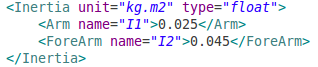
\includegraphics[scale=0.5]{XMLInertia.png}
\end{flushleft}

$<DampingTerm>$ is composed of $<bi>$ element where $i$ is the number of the damping term. Each of these elements contains a float.
\begin{flushleft}
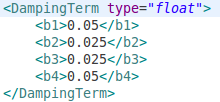
\includegraphics[scale=0.5]{XMLDamping.png}
\end{flushleft}

$<MomentMatrix>$ is composed of $<mi>$ elements where $i$ is the number of the moment element. Each of these elements contains a float.
\begin{flushleft}
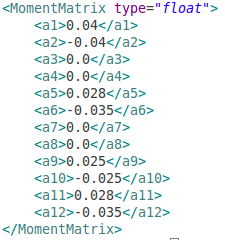
\includegraphics[scale=0.5]{XMLMoment.png}
\end{flushleft}

$<Bounds>$ is composed of one element per joint. The joint element is named with the joint name and contain a $<Lower>$ and an $<Upper>$ element for the lower and upper bounds.
\begin{flushleft}
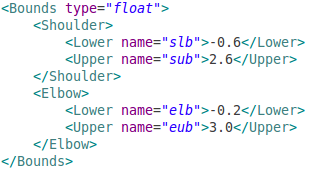
\includegraphics[scale=0.5]{XMLBounds.png}
\end{flushleft}
\subsubsection{Muscles setup}
The name of the structure setup file is "MusclesParamsDM.xml" where D is the number of degrees of freedom of the arm and M the number of muscles.
The root element is $<Muscle>$ and it is composed of two elements: $<MaximumForce>$ and $<Knoise>$.

$<MaximumForce>$ contains an element per muscle. These elements contain the maximun force of the related muscle.
\begin{flushleft}
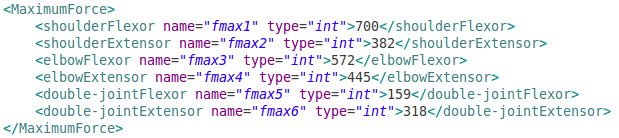
\includegraphics[scale=0.5]{XMLForce.png}
\end{flushleft}
The $<Knoise>$ element contains a float that is the noise parameter for the muscle activations.
\begin{flushleft}
\includegraphics[scale=0.5]{XMLKnoise.png}
\end{flushleft}
Is it truly deprecated?

\subsection{Global setup}
\label{global}
The root of this setup file is $<setup>$. It is composed of 10 elements.

$<data>$ elements contain data information: the size of the input, the size of the output, and if there is noise or not. 
The Arm module used is determined by the input or the output size (the size of the input is two times the number of joints and the size of the output is the number of muscles). Only the Arm with two joints and six muscle have been tested.

The next element is $<regression>$, it contains parameters of the regression module used. Its elements are the regression elements used (curently RBFN or NeuralNet), $<thetaFile>$ for the name of output parameters file and $<resultPath>$ for the directory where the result is saved.

\subsubsection*{RBFN}
The $<RBFN>$ elements is composed of $<nbFeatures>$, $<lambda>$ and $<fromStruct>$.
\begin{itemize}
\item
$<nbFeatures>$ is the number of features, it is an integer.
\item
$<lambda>$ is a float
\item
$<fromStruct>$ is a string (``yes'' or ``no'') meaning if it uses a structure from a previous RBFN or a new.
\end{itemize}

\subsubsection*{NeuralNet}

The $<NeuralNet>$ element is composed of $<inputLayer$, $<hiddenLayers>$, $<outputLayers>$, $<bias>$, $<learningrate>$ and $<momentum>$.
$<hiddenLayers>$ are compose of zero or any number of $<hiddenLayer>$ we want. 
Each layer element contains an element type, the different type are described in the Neural Network section. 
Furthermore, $<hiddenLayer>$ has a $<size>$ element that contain the size of the layer. 
The size of the input and output layers are the input and output data size.
$<bias>$ is a string (``yes'' or ``no'') meaning if it uses a bias or no. 
$<learningrate>$ and $<momentum>$ are float numbers.
\begin{flushleft}
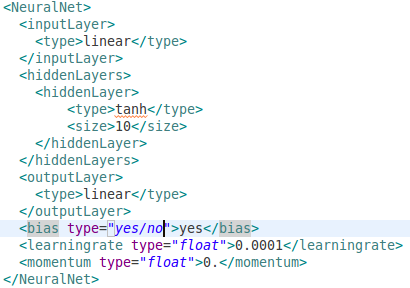
\includegraphics[scale=0.5]{XMLNeuralNet.png}
\end{flushleft}
The next element is $<costFunction>$, it contains the parameters of the cost function : gamma, rho and upsilon and the used python classes.
\begin{flushleft}
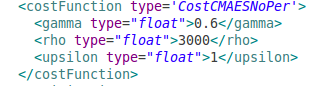
\includegraphics[scale=0.5]{XMLCost.png}
\end{flushleft}
Then we have the $<optimization>$ element that has an attribute type, for the type of the optimization done (CMAES or DDPG). 
For both types, we have elements $<maxIteration>$, $<numberRepetition>$, $<resultPath>$.
Furthermore for the CMAES type, we have two other elements $<sigma>$ and $<popsize>$.
\begin{flushleft}
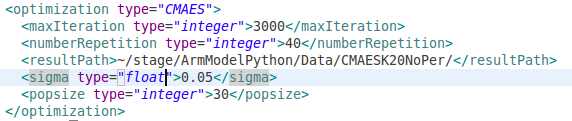
\includegraphics[scale=0.5]{XMLOpti.png}
\end{flushleft}
Then we have the target information (size and coordinates).
\begin{flushleft}
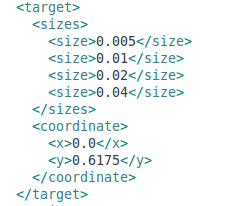
\includegraphics[scale=0.5]{XMLTarget.png}
\end{flushleft}
The trajectory information, $<initialPosition>$ is the name of the file that contains the coordinate of the initial points of the trajectory.
\begin{flushleft}
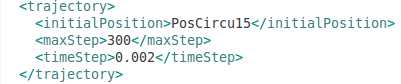
\includegraphics[scale=0.5]{XMLTraj.png}
\end{flushleft}
In the estimation element, we find the type of the estimation and the delay.  
\begin{flushleft}
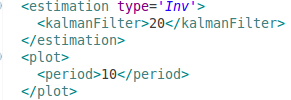
\includegraphics[scale=0.5]{XMLEstim.png}
\end{flushleft}

\section{Overview of the packages}

\subsection{ArmModel}
The ArmModel package contains all the files related to the arm model, 
Arm.py is an abstract class, the arm model needs to inherit from it. 
Arm26.py and Arm38.py are the arm model already implemented. The *XML.py file parse the * setup file in ArmModel/Setup.

\subsection{Cost}
This package contains all different cost implemented. CostType is a dictionary of all costs.

\subsection{DDPG}
This package contains the DDPG algorithm.

\subsection{Experiment}
This package contains all different state estimator, there are referenced in StateEstimatorType. 
TrajMaker.py contains the tools to compute one trajectory, Experiments.py use TrajMaker to run all trajectories.

\subsection{Main}
In MainCMAES.py (resp. MainDDPG.py) we found all the operations for the optimization with CMAES (resp. DDPG).

\subsection{Optimizer}
This package contains the DDPG environments and the Bayesian Optimization. For more detail about Bayesian optimization, see 
\url{https://github.com/fmfn/BayesianOptimization} 

\subsection{Plot}
This package contains the plot functions.

\subsection{Regression}
This package contains the regression classes, all regression classes have to inherit from Regression.py.
DataSet.py is used to handle a data set, and RunRegression to handle a regression algorithm.

\subsection{Utils}
In this package, we find several tools, like standard and xml files readers, the chronometer and a distribution comparator.

\end{document}
